
\documentclass[11pt]{article}
\usepackage{graphicx}
\usepackage{float}

\begin{document}
\title{ LiFePO$_4$: calculation of structural properties \\ of material with H-defects\\ 
\large Final project }
\author{Irina Varlamova}
\maketitle

\section{Computational Chemistry}
\noindent\mbox{\textbf{Introduction}}

Batteries are being developed to power an increasingly diverse range of applications, like cars, electrical vehicles, electromic devices, microchips, systems for electrochemical energy storage and other. Such electronic components are often seen as being the heaviest, costliest and least environmentally friendly and most demanding to development despite their simple design concept. All batteries are composed by two electrodes: anode and cathode and separated layes berween them - electrolyte, it is an ion-conductive material. Anode and cathode have different chemical potentials, which are dictated by chemistry of each. There can be observed the important paremeters of batteries. First of all, it is electrical energy per mass, which is presented as a function of the cell's voltage and capacity, which are dependent on the chemistry of the system. Another parameter is power of battery, which also crucially depends on the chemistry of the battery contains. Thus, the chemical composition of the batteries electrodes has significant influence to their electrochemical properrties. Hundreds of electrochemical couples were proposed during the development of this fiels of technology. 

Olivine - is one of the most common minerals on earth, forms a group of compounds with a formula M$_2$XO$_4$ (M = Li, Na, Zn and others;  = P, Si). Such olivine structure consists of a hexagonal close packing of oxygen with M atoms in half of the octahedral sites and X atoms in 1/8 of the tetrahedral sites and space group of crystal is presented as $Pnma$. Olivine-structured orthophosphates Li$M$PO$_4$ ($M$ is transition metals) have such crystallographic features and became a widely used as a cathode materials due to their good thermal stability and high voltage.  In this application lithium-iron phosphate LiFePO$_4$ is more popular and widely used in the electrochemical industry due to high Li-ion conductivity and low cost and this material \cite{LFP}. But, despite its extensive study and use, there are many questions about defects of the structure and their impact on the electrochemical properties.

Lithium anti-site (Li-Fe) defect is more investigated. Such defect provides slow Li-ion diffusion on [010] channel and Li-ion diffusion becomes more isotropic as the concentration of anti-site defects increase \cite{LiFe}. Another type of observed defect of LiFePO$_4$ is lithium-vacancy, which can provide better ion-conductivity of cathode despite the more high formation energy (compared with Li-Fe exchange defect) \cite{Livac}. Also, there can be observed OH-defects, which are characteristic of many olivine materials. Since the hydrothermal synthesis is one of the most effective and common method of Li$M$PO$_4$ production so the OH-defects are intrinsic for LiFePO$_4$ \cite{def}, but formation mechanics and properties of such defective material are not fully studied \cite{def1}. In case of OH formation mechanism like in Mg$_2$SiO$_4$ system, where is observed the replace of Si vacancy with four hydrogen type defects \cite{oh}. Such OH-defects also provide an impact to ionic and electronic conductivity of cathode material, intercalation potential of lithium, phase transition mechanism and thermal stability of structure.

As part of this work the influence of OH-defect formation in LiFePO$_4$ to its structural properties is investigated. There were observed the H atom in free octahedral and tetrahedral position of structure, diffusion path of such different position of defects and OH-compound in P-vacancy position. Such violations in the cathode structure can provide new electrochemical and functional properties, thus, investigate of defects can give new ability for batteries. Obviously, the presence of hydroxide-ions in the structure of cathode material affects to the ionic and electronic conductivity. In this application, the phase transformation mechanism, the stable region of LiFePO$_4$ and possible charge/discharge mechanism are more interest.

\noindent\mbox{\textbf{Computational method}}

The calculations were carried out using density functional theory (DFT) with general gradient approximation (GGA) for exchange-correlation energy. The energy cutoff was 400eV and k spacing 0.3 (or 0.15 for band structure calculations), Fermi level is smeared by the Gaussian method.

\noindent\mbox{\textbf{Results}}

This work is aimed to study the defects in LiFePO$_4$ cathode material. The calculation of structural and electronic properties of LiFePO$_4$ is the first stage of this work. First of all, the space group of crystal is $Pnma$, the Wyckoff position of atoms are presented in Table \ref{tabular:wyckoff}.  As it was described above, structure of LiFePO$_4$ consist of a hexagonal close packing of oxygen with Li and Fe located in half of the octahedral sites and P in 1/8 of tetrahedral sites. The FeO$_6$ disorted octahedra are corner shared and cross linked by the PO$_4$ groups, forming a three-dimentional network with perpendicular tunnels along the [001] direction \cite{morgan}. 

\begin{table}[H]
\caption{$Pnma$ Wyckoff position of atoms}
\label{tabular:wyckoff}
\begin{center}
\begin{tabular}{|c|c|c|}
\hline
& & \\
 \textbf{The Wyckoff parameter} & \textbf{Element}  & \textbf{Coordinates}  \\
\hline
& & \\
8 d & O3 & $\pm$(x, y, z), $\pm$(x, 1/2-y, z), \\ 
  &  &  $\pm$ (x+1/2, 1/2-y, 1/2-z), \\
 &  &  $\pm$(x+1/2, y, 1/2-z)  \\
\hline
& & \\
4 c & Fe, P, O1, O2 & $\pm$($u$+1/2, 1/4, 1/2-$v$), \\
&  &   $\pm$($u$, 1/4, $v$) \\
\hline
& & \\
4 b & - & \\
\hline
& & \\
4 a & Li & (0, 0, 0), (1/2, 0, 1/2), \\
  &  &  (0, 1/2, 0), (1/2, 1/2, 1/2) \\
\hline
\end{tabular}
\end{center}
\end{table}


First step of study is structural optimization of crystal. As it can be seen from Fig.\ref{tabular:str}, for LiFePO$_4$ the cell compression (decrease of cell parameters) is observed. 

\begin{figure}[H]
\begin{minipage}[h]{0.5\linewidth}
\begin{tabular}{ccc}
Parameter & Initial & Optimized \\
a, \AA & 10.45 & 9.88 \\
b, \AA & 6.09 & 5.79 \\
c, \AA & 4.75 & 4.66 \\
$\alpha$=$\beta$=$\gamma$ & 90 & 90 \\
& & \\
\end{tabular}
\end{minipage}
\hfill
\begin{minipage}[h]{0.35\linewidth}
\center{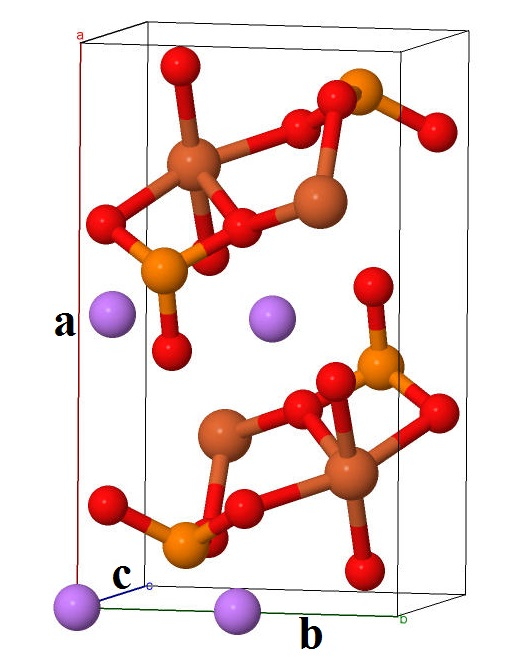
\includegraphics[width=0.7\linewidth]{out.jpg}}
\end{minipage}
\caption{Structure parameters of LiFePO$_4$ before and after geomentry optimization}
\label{tabular:str}
\end{figure}

The band structure and density of states (DOS) characterization with respect to Fe atom are provided in Fig.\ref{dos}. As it can be seen the maximum of valence band is formed by d-electrons and the minimum of conductive band from s-electrons of Fe. Band gap of LiFePO$_4$ has the value of 3.6eV, which is in good agreement with references \cite{bgap}.

\begin{figure}[H]
\begin{minipage}[h]{1\linewidth}
\center{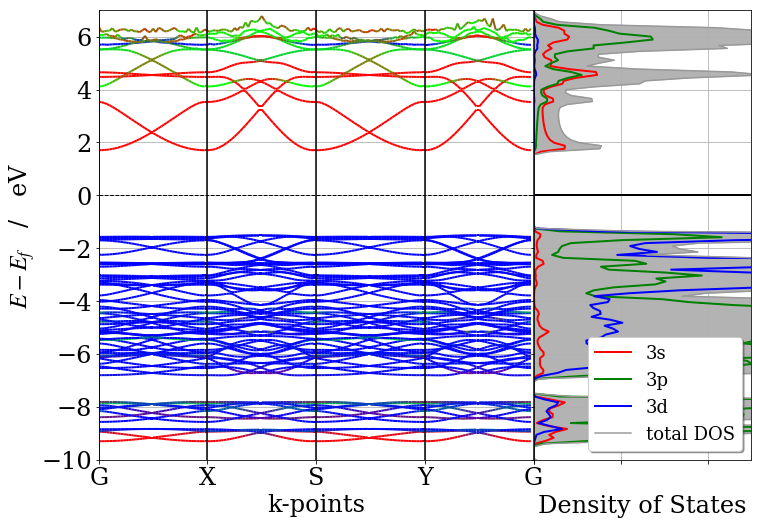
\includegraphics[width=1\linewidth]{band.png}}
\end{minipage}
\caption{Band structure and DOS of LiFePO$_4$ in related to Fe}
\label{dos}
\end{figure}

As it can be observed from Table \ref{tabular:wyckoff}, the 4b Wyckoff position of LiFePO$_4$ is not occupied. Thus, for study of intercalation defect in octahedral environment of oxygen atoms, there can be put hydrogen atom to one of this non-occupied position. Also, there can be the H-defect in tetrahedral environment of oxygen. To investigate the hydrogen point defect in different position there was provided structure optimization of 1$\times$2$\times$2 LiFePO$_4$ with intercalation H-atom, Fig.\ref{tabular:def}. During optimization of structure with H-additional atom, there observed some change of atoms positions. In case of octahedral environment of hydrogen atom there are observed the increase of the pore with hydrogen atom volume, the hedrogen in tetrahedral positions tends to leave the tetrahedral environment, Table \ref{tabular:change}.

\begin{figure}[H]
\begin{minipage}[h]{0.3\linewidth}
\center{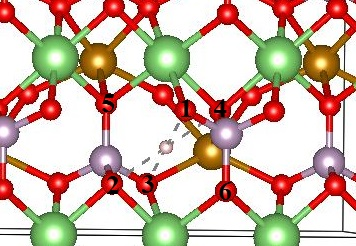
\includegraphics[width=1\linewidth]{oct.jpg}}
\end{minipage}
\hfill
\begin{minipage}[h]{0.3\linewidth}
\center{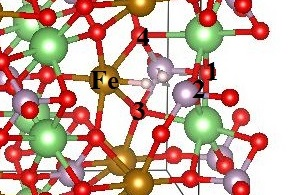
\includegraphics[width=1\linewidth]{tet1.jpg}}
\end{minipage}
\hfill
\begin{minipage}[h]{0.3\linewidth}
\center{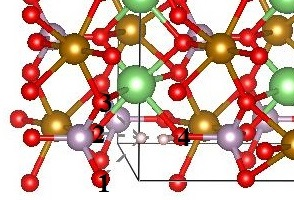
\includegraphics[width=1\linewidth]{tet22.jpg}}
\end{minipage}
\caption{Octahedral and two types tetrahedral defect position of hydrogen atom}
\label{tabular:def}
\end{figure}

\begin{table}[H]
\footnotesize{
\caption{The change of bond lenghs in defective LiFePO$_4$}
\label{tabular:change}
\begin{center}
\begin{tabular}{|c|c|c|c|}
\hline
& & & \\
 \textbf{ } & \textbf{octahedral (in/opt)}& \textbf{tetrahedral1 (in/opt)}  & \textbf{tetrahedral2 (in/opt)}  \\
\hline
& & & \\
(x, y, z) & (0.0, 0.5, 0.25) / &  (0.89, 0.37, 0.07) /  & (0.1, 0.12, 0.0) /  \\ 
 & (0.0, 0.5, 0.25)  &   (0.82, 0.37, 0.07) & (0.14, 0.12, 0.93) \\ 
\hline
& & & \\
H-O1, \AA & 1.98 / 2.09 &  1.75 / 3.06 & 1.97 / 2.39 \\ 
\hline
& & & \\
H-O2, \AA & 1.98 / 2.09 & 1.94 / 1.58 & 2.06 / 2.82 \\
\hline
& & & \\
H-O3, \AA & 1.85 / 2.06 & 1.45 / 2.44 & 1.97 / 2.39 \\
\hline
& & & \\
H-O4, \AA & 1.85 / 2.06 & 1.45 / 2.44 & 1.35 / 1.05 \\
\hline
& & & \\
H-O5, \AA & 2.12 / 2.20 &  &  \\
\hline
& & & \\
H-O6, \AA & 2.12 / 2.20 & & \\
\hline
& & & \\
H-Fe, \AA &  & 4.27 / 1.48 &  \\
\hline
\end{tabular}
\end{center}
}
\end{table}

In case of formation energy discussion, there can be observed the lowest energy after optimization of H-defect in tetrahedral positions, Fig.\ref{foren}.

\begin{figure}[H]
\begin{minipage}[h]{1\linewidth}
\center{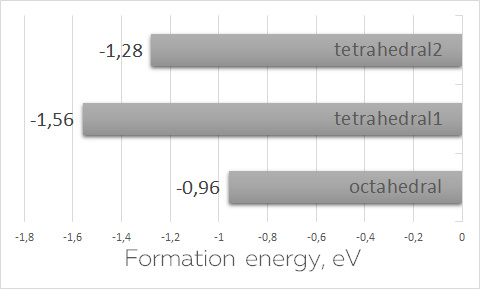
\includegraphics[width=1\linewidth]{foren.png}}
\end{minipage}
\caption{Formation energy of H-defects in compare with H$_2$ molecule}
\label{foren}
\end{figure}

In case of study of diffusion path between two probably vacancies (tetrahedral 1 and octahedral 5) there tetrahedral site is more favorable due to its minimum of formation energy, Fig.\ref{difpath}. 

\begin{table}[H]
\caption{The diffusion path of H-atom between tetrahedral (1) and octahedral (5) sites in defective LiFePO$_4$}
\label{tabular:difpath}
\begin{center}
\begin{tabular}{|c|c|c|c|}
\hline
& & \\
 \textbf{ } & \textbf{initial}& \textbf{optimized}  \\ 
\hline
& & \\
1 & (0.89, 0.12, 0.43) &  (0.87, 0.12, 0.43) \\ 
\hline
& & \\
2 & (0.90, 0.09, 0.38) & (0.91, 0.09, 0.36) \\
\hline
& & \\
3 & (0.94, 0.06, 0.34) & (0.91, 0.06, 0.29) \\
\hline
& & \\
4 & (0.97, 0.03, 0.29) & (0.99, 0.04, 0.29) \\
\hline
& & \\
5 & (1.0, 0.0, 1.25) &  (0.0, 0.0, 0.25)  \\
\hline
\end{tabular}
\end{center}
\end{table}

\begin{figure}[H]
\begin{minipage}[h]{1\linewidth}
\center{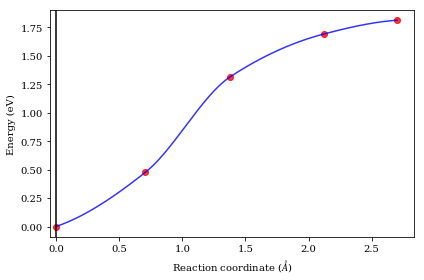
\includegraphics[width=0.8\linewidth]{difpath.png}}
\end{minipage}
\caption{Energy difference of the diffusion path of H-atom defect between tetrahedral and octahedral vacansies in LiFePO$_4$}
\label{difpath}
\end{figure}

Finally, this work is aimed to study the defects also in P-vacancy position. In such case of defect there can be observed the change of P-atom with 1, 2, 3 or 4 atoms of hydrogen. During this work the study of four atoms of H in P-atomic position was studied in case of three relative positions: four H-atoms inside the tetrahedron oxide invironment, one of H-atom outside the tetrahedron and two H-atoms outside the terahedron, Table \ref{Ppos}. This table describes the case of close placement of hydrogen atoms to oxygen (less than 0.9 \AA). In all of three positions of hydrogen atoms there are observed the bond between two or three hydrogen atoms inside the crystal with H$_2$ or H$_3$ molecules creating, Fig.\ref{h2}, \ref{h3}. Probably, such binding effect of hydrogen atoms is due to the repulsion between hydrogen and oxygen atoms due to a short connection between them and the predominance of repulsive forces.

\begin{table}[H]
\scriptsize{
\caption{Bond lenght between O and H-atoms in pore of P-vacancy of LiFePO$_4$}
\label{Ppos}
\begin{center}
\begin{tabular}{|c|c|c|c|}
\hline
& & & \\
 \textbf{ } & \textbf{H inside (in/out)}& \textbf{one H outside (in/out)} & \textbf{two H outside (in/out)} \\ 
\hline
& & & \\
H-O1, \AA & 0.74/1.62 & 0.74/1.75 & 0.74/1.97\\ 
\hline
& & & \\
H-O2, \AA & 0.74/1.81 & 0.74/1.95 & 0.74/1.75 \\
\hline
& & & \\
H-O3, \AA & 0.78/0.98 & 0.97/0.97  & 0.97/0.97 \\
\hline
& & & \\
H-O4, \AA & 0.84/0.99 & 0.84/0.99 & 0.81/1,78 \\
\hline
& & & \\
GS energy, eV & -786.5 & -787.4 & -784.9 \\
\hline
& & & \\
to note & H$_2$ molecule in the crystal & H$_2$ molecule in the crystal & H$_3$ molecule in the crystal \\
\hline
\end{tabular}
\end{center}
}
\end{table}

\begin{figure}[H]
\begin{minipage}[h]{0.48\linewidth}
\center{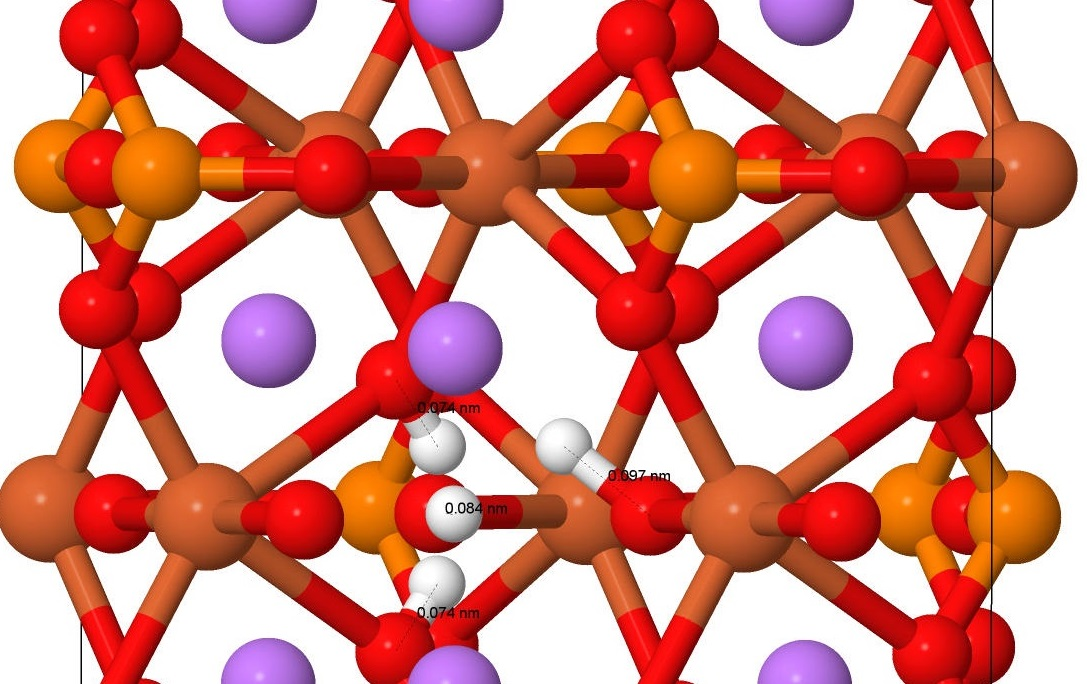
\includegraphics[width=0.9\linewidth]{in2.jpg}}
\end{minipage}
\hfill
\begin{minipage}[h]{0.48\linewidth}
\center{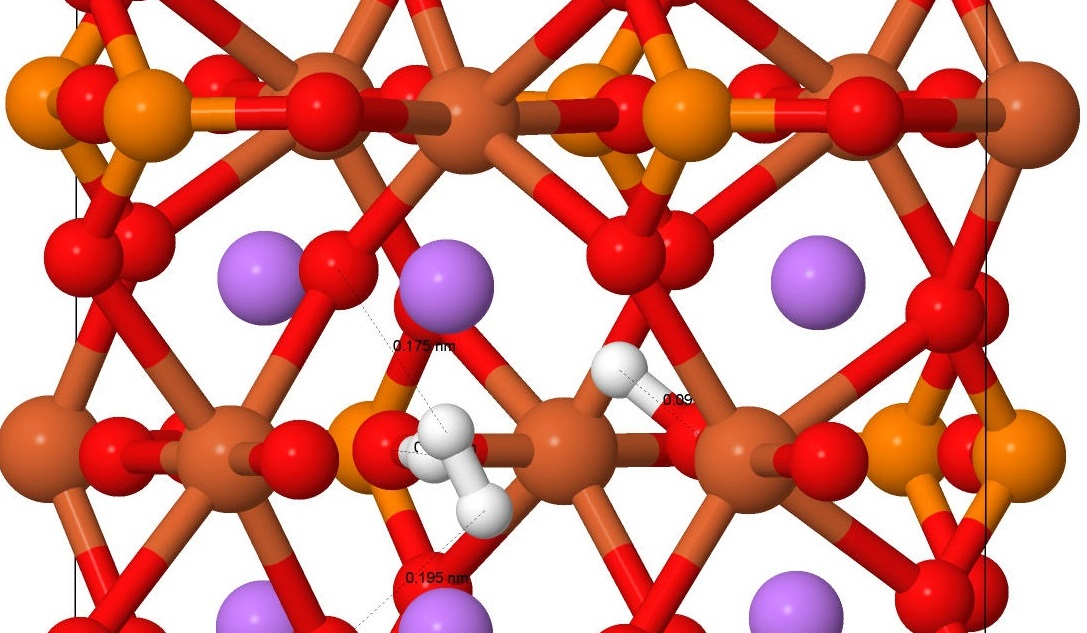
\includegraphics[width=1\linewidth]{out2.jpg}}
\end{minipage}
\caption{H$_2$ molecule inside of P-vacancy of LiFePO$_4$ before and after optimization}
\label{h2}
\end{figure}

\begin{figure}[H]
\begin{minipage}[h]{0.48\linewidth}
\center{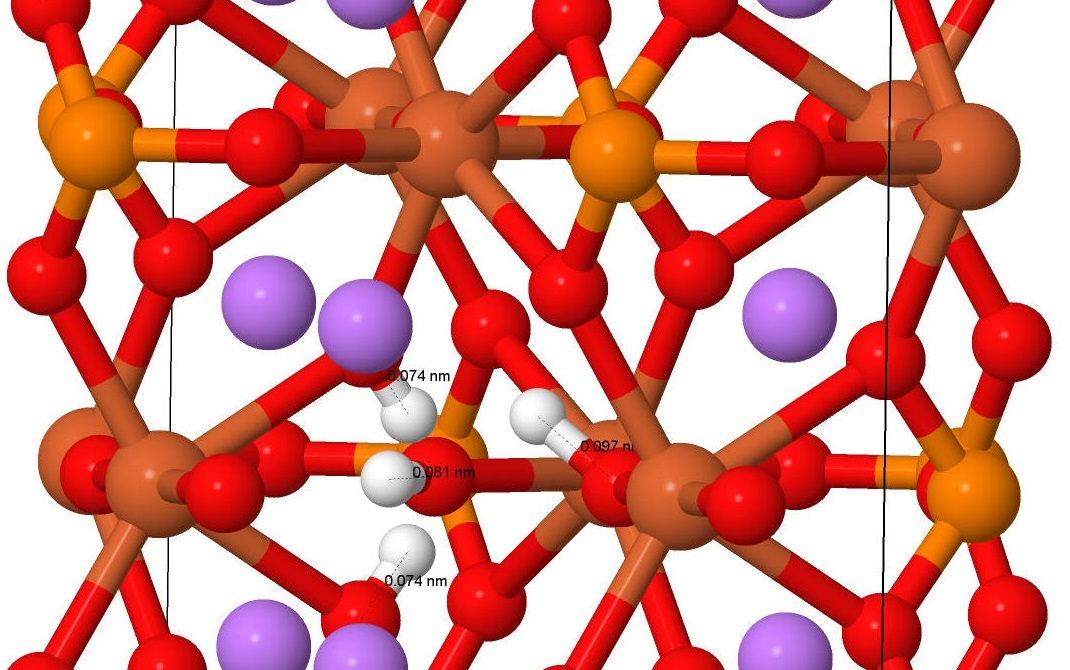
\includegraphics[width=0.9\linewidth]{in3.jpg}}
\end{minipage}
\hfill
\begin{minipage}[h]{0.48\linewidth}
\center{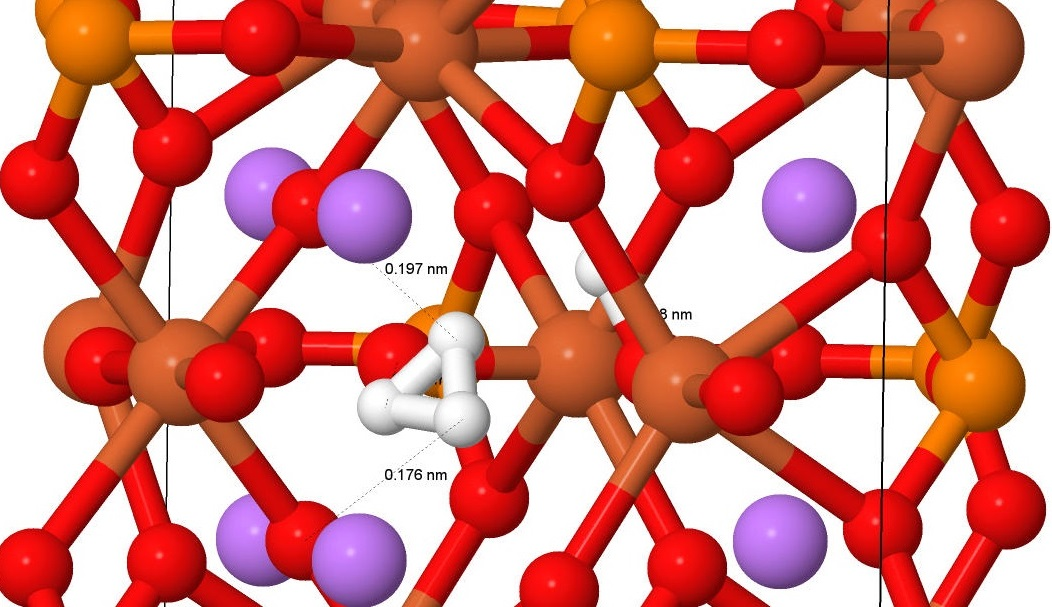
\includegraphics[width=1\linewidth]{out3.jpg}}
\end{minipage}
\caption{H$_3$ molecule inside of P-vacancy of LiFePO$_4$ before and after optimization}
\label{h3}
\end{figure}

In case of larger length between oxygen and hydrogen atoms another placement of hydrogen atoms is observed after optimization, Fig. \ref{h21}, \ref{h31}. There the legth of O-H bond is approximately 0.97-1\AA $ $ in all cases of H placement and there are not H$_2$ or H$_3$ molecules inside the crystal. There are not repulsive forces between oxygen and hydrogen atoms. Also Table \ref{Ppos} and \ref{Ppos1} are provided the ground state energies, which is correspond about more stable solution in compound with 0.97-1\AA$ $ length between O and H atoms.

\begin{table}[H]
\scriptsize{
\caption{Bond lenght between O and H-atoms in pore of P-vacancy of LiFePO$_4$}
\label{Ppos1}
\begin{center}
\begin{tabular}{|c|c|c|c|}
\hline
& & & \\
 \textbf{ } & \textbf{H inside (in/out)}& \textbf{one H outside (in/out)} & \textbf{two H outside (in/out)} \\ 
\hline
& & & \\
H-O1, \AA & 0.96/0.97 & 0.96/0.98 & 0.96/0.98 \\ 
\hline
& & & \\
H-O2, \AA & 1.01/0.98 & 1.01/1.00 & 1.01/1.01 \\
\hline
& & & \\
H-O3, \AA & 0.95/0.97 & 1.08/0.98  & 1.08/0.98  \\
\hline
& & & \\
H-O4, \AA & 1.03/0.97 & 1.03/0.98 & 1.00/0.98 \\
\hline
& & & \\
GS energy, eV & -789.8 & -790.3 & -790.3 \\
\hline
\end{tabular}
\end{center}
}
\end{table}

\begin{figure}[H]
\begin{minipage}[h]{0.48\linewidth}
\center{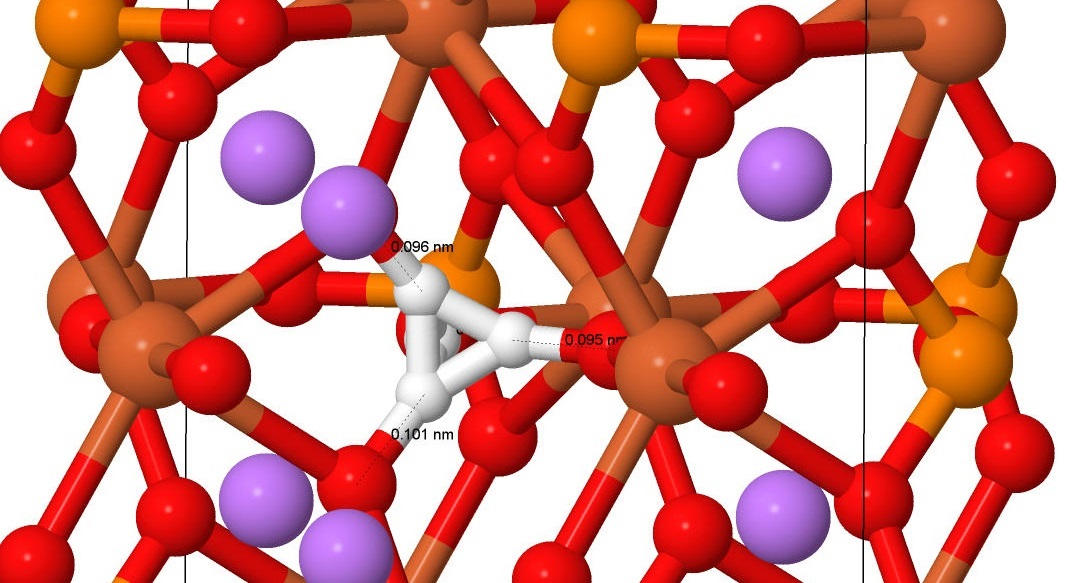
\includegraphics[width=0.85\linewidth]{in11.jpg}}
\end{minipage}
\hfill
\begin{minipage}[h]{0.48\linewidth}
\center{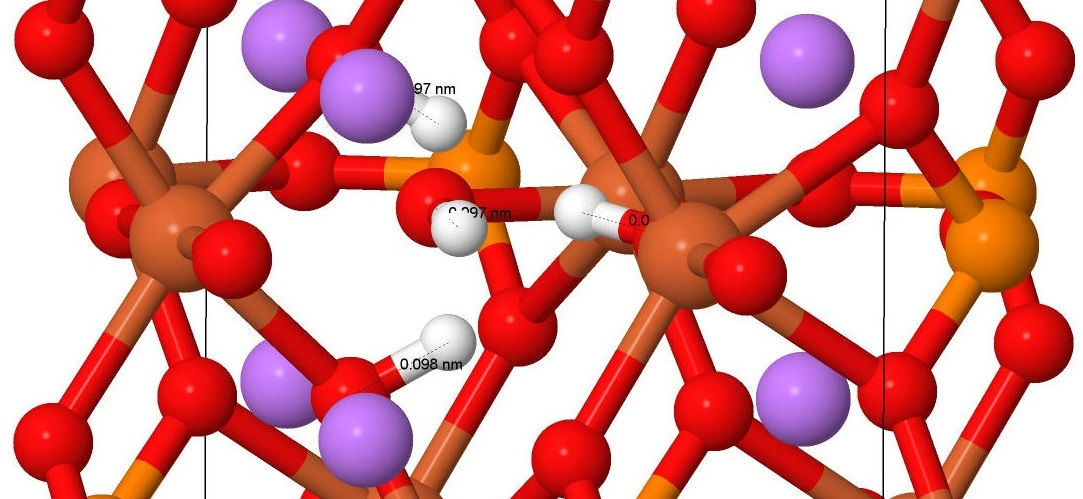
\includegraphics[width=1\linewidth]{out11.jpg}}
\end{minipage}
\caption{H-defect inside of tetrahedral P-vacancy of LiFePO$_4$ before and after optimization}
\label{h21}
\end{figure}

\begin{figure}[H]
\begin{minipage}[h]{0.48\linewidth}
\center{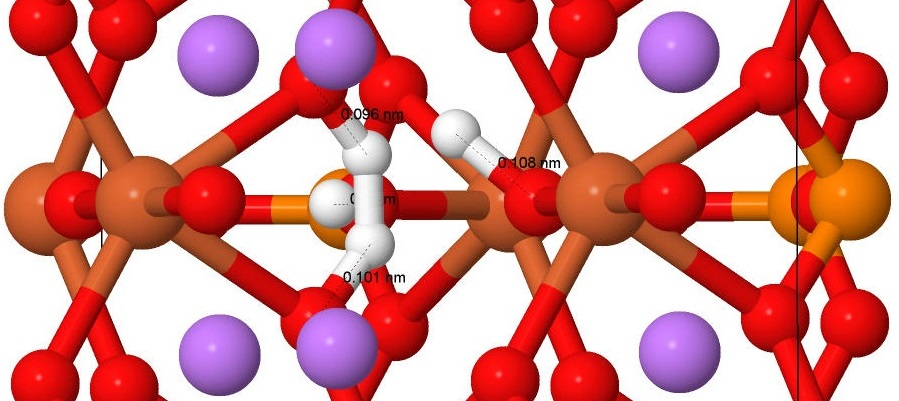
\includegraphics[width=1\linewidth]{in31.jpg}}
\end{minipage}
\hfill
\begin{minipage}[h]{0.48\linewidth}
\center{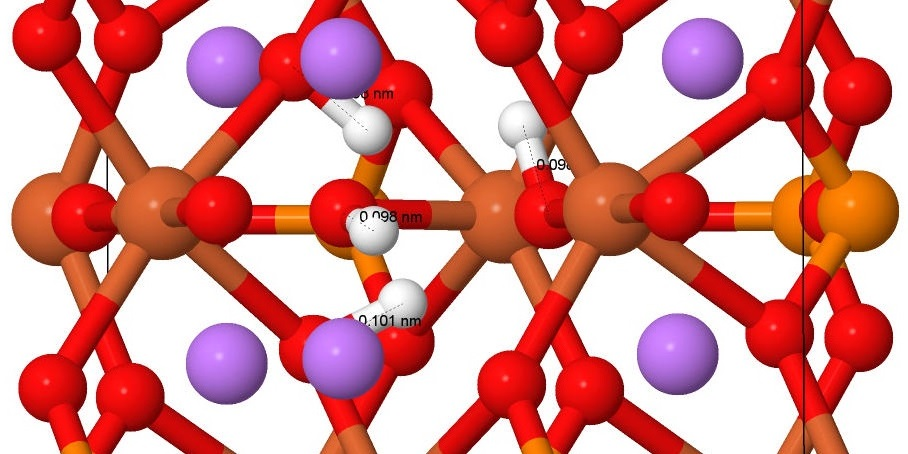
\includegraphics[width=0.9\linewidth]{out31.jpg}}
\end{minipage}
\caption{Two H-vacancy  outside of tetrahedral P-vacancy of LiFePO$_4$ before and after optimization}
\label{h31}
\end{figure}

Thus, this work provided three possible locations of hydrogen atoms defects in solid LiFePO$_4$: unoccupied tetrahedral and octahedral position and phosphorus vacancy in crystal. There were studied the possible ground state solutions and energy. But for complete study it is neseccary to investigate all possible positions (with different lengths and angles between internal and external atoms) for find a global minimum of energy.

\newpage

\section{ISP research project}

During ISP period the studies of LiFePO$_4$ defect structure on three main research direction were performed:

1. Structure stability of four H-atoms in P-vacancy in tetrahedral oxygen environment;

2. Structure stability of two H-atoms in Li-vacancy in octahedral oxygen environment;

3. Hydrogen grid of possible position of four H-atom in P-vacancy tetrahedral polyhedra and study of structural features of material.

\noindent\mbox{\textbf{Four H-atoms in P-vacansy of tetrahedral polyhedra}}

\begin{figure}[H]
\begin{minipage}[h]{0.3\linewidth}
\center{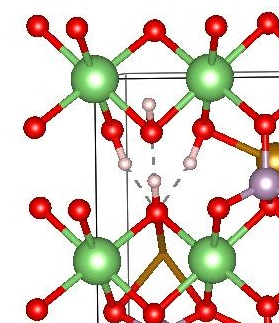
\includegraphics[width=0.85\linewidth]{1P4H.jpg}} Conf.1 \\
\end{minipage}
\hfill
\begin{minipage}[h]{0.3\linewidth}
\center{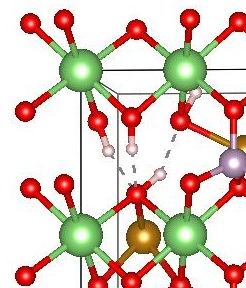
\includegraphics[width=0.85\linewidth]{2P4H.jpg}} Conf.2 \\
\end{minipage}
\hfill
\begin{minipage}[h]{0.3\linewidth}
\center{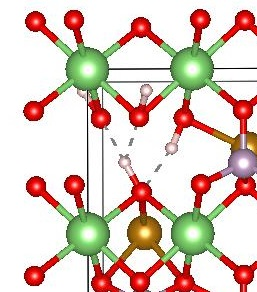
\includegraphics[width=0.85\linewidth]{3P4H.jpg}} Conf.3 \\
\end{minipage}
\vfill
\begin{minipage}[h]{0.3\linewidth}
\center{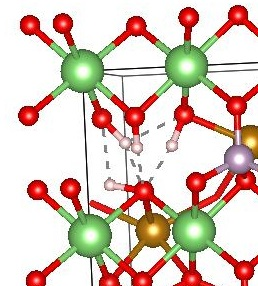
\includegraphics[width=0.85\linewidth]{4P4H.jpg}} Conf.4 \\
\end{minipage}
\hfill
\begin{minipage}[h]{0.3\linewidth}
\center{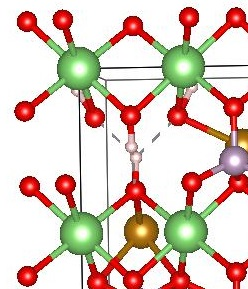
\includegraphics[width=0.85\linewidth]{5P4H.jpg}} Conf.5 \\
\end{minipage}
\hfill
\begin{minipage}[h]{0.3\linewidth}
\center{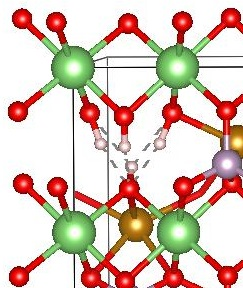
\includegraphics[width=0.85\linewidth]{6P4H.jpg}} Conf.6 \\
\end{minipage}
\vfill
\begin{minipage}[h]{0.3\linewidth}
%\center{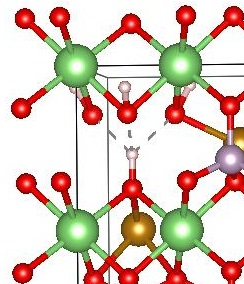
\includegraphics[width=0.85\linewidth]{7P4H.jpg}} Conf.7 \\
\end{minipage}
\hfill
\begin{minipage}[h]{0.9\linewidth}
\center{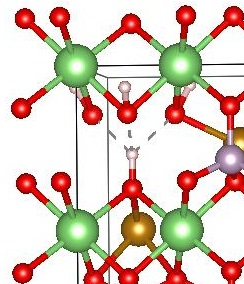
\includegraphics[width=0.3\linewidth]{7P4H.jpg}} Conf.7 \\
\end{minipage}
\caption{Configurations of (4H)$_{P}$ defects}
\label{pvac7}
\end{figure}

There is the article with investigating the defects in similar olivine structure of Mg$_2$SiO$_4$, \cite{mineral}. In this work the possible positions of four H-atoms in tetrahedral polyhedra with phosphorous vacancy was modeling and the stable solution was finding. Repeating similar reasoning in case of LiFePO$_4$ the stable (first) and non-stable (seventh) positions of hydrogen atoms were find, and these results are in good agreement with article,  Table \ref{4H}. But these are preliminary results because the structures need additional stage of optimization due to the presence of excess pressure in the structure. 

\begin{table}[H]
\scriptsize{
\caption{Possible positions of four H-atoms in phosphorus defect polyhedra}
\label{4H}
\begin{center}
\begin{tabular}{|c|c|c|c|}
\hline
& & & \\
 \textbf{Configuration num.} & \textbf{Energy (1 step), eV} &  \textbf{Energy (2 step), eV} &  \textbf{E$_{conf}$-E$_{conf2}$, eV}\\ 
\hline
&  & & \\
1  & -790.31 & -790.36 & 0.2\\ 
\hline
&  & &\\
2  & -789.40 & -790.56 & 0.0\\
\hline
&  & &\\
3 & -790.17 & -790.27 & 0.03\\
\hline
&  & &\\
4 & -789.35 & -790.34 & 0.22\\
\hline
&  & &\\
5 & --788.85 & -790.03 & 0.53\\
\hline
&  & &\\
6 & -790.05 & -790.01 & 0.55\\
\hline
&  & &\\
7 & -789.71 & -789.87 & 0.69\\
\hline
\end{tabular}
\end{center}
}
\end{table}

\noindent\mbox{\textbf{Structure stability of two H-atoms in Li-vacancy in octahedral oxygen environment}}

In case of hexagonal vacancy position (like Fe or Li) there can be observed the change of Li atom by one hydrogen and iron atom by two hydrogen. But in case of Li-vacancy there was some mistake and two hydrogen atoms in pore of lithium atom were modeling. Schematically such structure is presented in fig.\ref{livac}. Such types of defects are needed in more systematically study in the future.

\begin{figure}[H]
\begin{minipage}[h]{1\linewidth}
\center{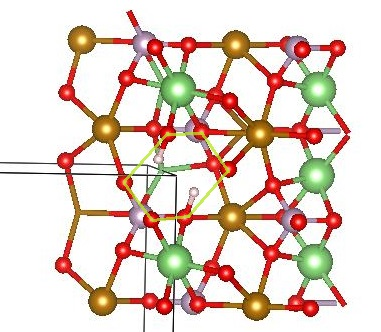
\includegraphics[width=0.5\linewidth]{Li_vac.jpg}}
\end{minipage}
\caption{ Two H-atoms in Li-vacancy octahedral polyhedra}
\label{livac}
\end{figure}

\noindent\mbox{\textbf{Grid of possible position of hydrogen atoms in P-vacancy}}

First of all. there is necessary to create the analitical formula of chemical reaction:

\begin{equation}
\frac{1}{4}O_2 + \frac{1}{2}H_2O + 16 Li^{+}Fe^{2+}P^{5+}O^{2-}_4 = Li^{+}_{15}Fe^{2+}_{16}P^{5+}_{16}O^{2-}_{64} + LiOH
\label{firstreaction}
\end{equation}

\begin{equation}
H_2O + Li^{+}_{15}Fe^{2+}_{16}P^{5+}_{16}O^{2-}_{64} + LiOH = H^{+}_{4}Li^{+}_{16}Fe^{2+}_{15}Fe^{3+}_{1}P^{5+}_{15}O^{2-}_{64} + Li_3PO_4 + H_2O
\label{secondreaction}
\end{equation}
There can be observed the formation of Li defect in water and oxygen environment, (\ref{firstreaction}) and P-defect formation with four hydrogen atoms in pore, (\ref{secondreaction}).

In this case there were observed the possible positions of H-atoms in tetrahedral polyhedra with P-vacancy. There are three different positions of oxygen atoms (in depend of environmental atoms) around which there was build the grif of hydrogen, fig. \ref{PH1}-\ref{PH3}. There can be observed two parallen planes along XY-surface with different atoms: in fig.\ref{PH1} iron atom is located in first plane, two lithium atoms are located in second plane; in fig.\ref{PH2} all atoms - two lithium and one iron, are located in first plane, when second plane has only oxygen atoms with empty polyhedral; in fig.\ref{PH3} one iron atom is located in first plane and one iron with one lithium in second plane. Thus, the structure of environment of oxygen atoms is different, but there is one the same property: all oxygen atoms are surrounded by eight tetrahedral polyhedra (in pictures they are marked by gray numbers) and six octahedral polyhedra (marked by black numbers). The tetrahedral without P-atom is noted in fig.\ref{PH1} with 7 grey number, in  fig.\ref{PH2} with 8 grey number and  in fig.\ref{PH3} with 6 grey number. Other seven tetrahedral polyhedra are not occupied by some atoms in the original LiFePO$_4$ structure. Also each oxygen atoms are occupied by six octahedral polyhedra, three of which are occupied by iron or lithium (for example, in fig. \ref{PH1} it is 1, 5 and 6 black numbers) and three are free (in fig. \ref{PH1} it is 2, 3 and 4 black numbers).

The grid of distribution H-atoms represents the 'cloud' of H-atoms in all possible positions around oxygen, there is the condition on the distance between oxygen and hydrogen (more than 0.9\AA and less than 1.3\AA). To study the potential surface of such distribution of H-atoms near the oxygen atoms of phosphorus tetragonal polyhedra we can chose three different ways:

1. full optimization of geometry (but there are too much atoms around several hundred, that requires a lot of resources to calculation);

2. molecular dynamics calculation to find the potential barriers between possible stable positions;

3. non-relaxation solution of hydrogen atoms energies for first step of potential surface investigating.

In this conditions a non-relaxation way as a first step of potential investigating is in the performance. 
   

\begin{figure}[H]
\begin{minipage}[h]{0.5\linewidth}
\center{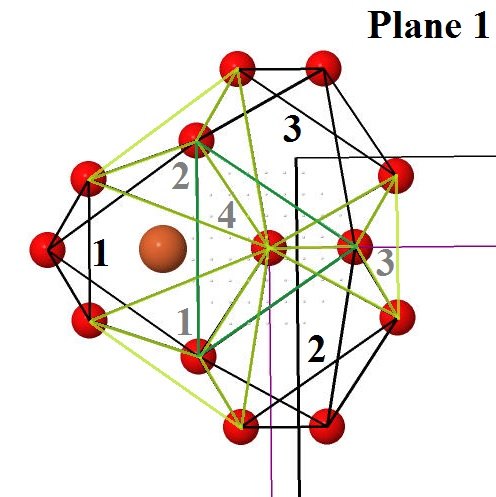
\includegraphics[width=0.8\linewidth]{O1_1.jpg}}
\end{minipage}
\hfill
\begin{minipage}[h]{0.5\linewidth}
\center{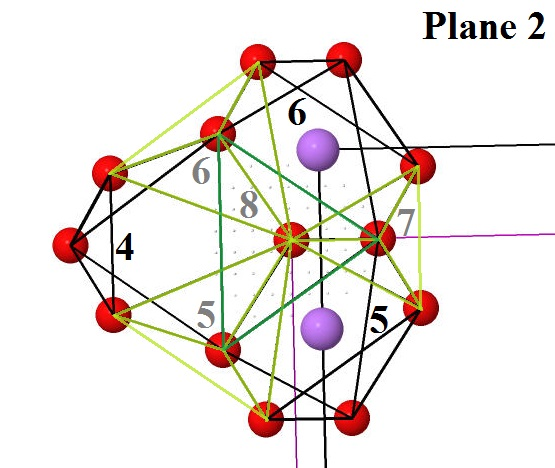
\includegraphics[width=0.85\linewidth]{O1_2.jpg}} 
\end{minipage}
\caption{ Polyhedra around O$_1$(-0.046, 0.125, 0.147) }
\label{PH1}
\vfill
\begin{minipage}[h]{0.5\linewidth}
\center{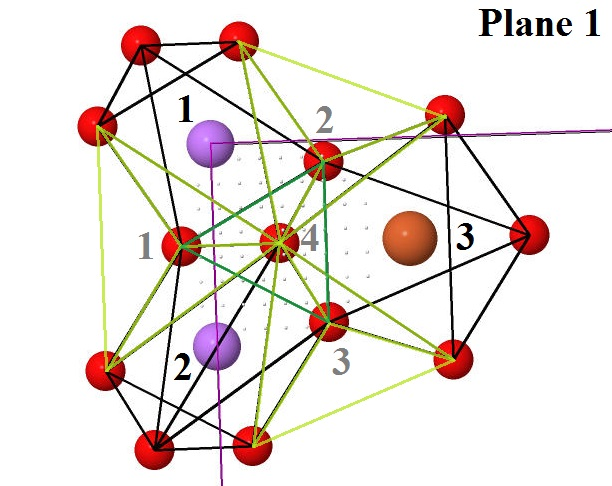
\includegraphics[width=0.85\linewidth]{O2_1.jpg}} 
\end{minipage}
\hfill
\begin{minipage}[h]{0.5\linewidth}
\center{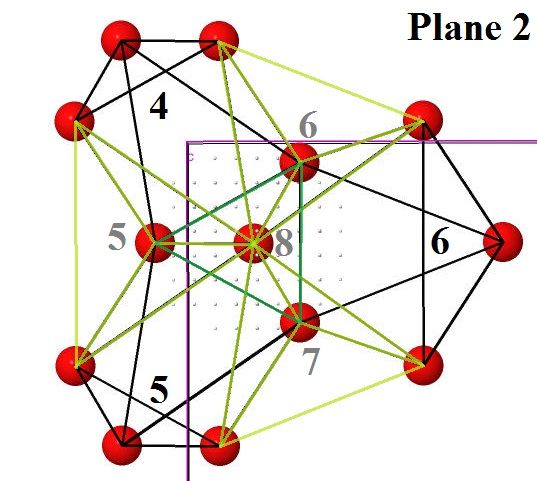
\includegraphics[width=0.72\linewidth]{O2_2.jpg}} 
\end{minipage}
\caption{ Polyhedra around O$_2$(0.095, 0.125, 0.370) }
\label{PH2}
\vfill
\begin{minipage}[h]{0.5\linewidth}
\center{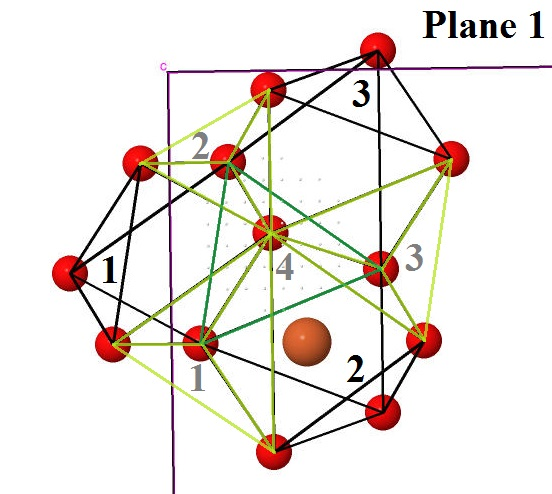
\includegraphics[width=0.85\linewidth]{O3_1.jpg}} 
\end{minipage}
\hfill
\begin{minipage}[h]{0.5\linewidth}
\center{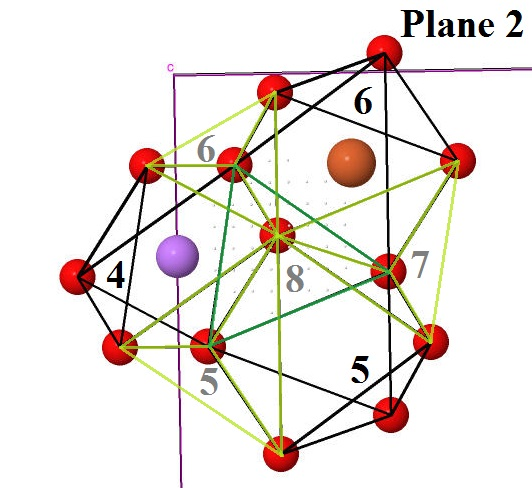
\includegraphics[width=0.85\linewidth]{O3_2.jpg}} 
\end{minipage}
\caption{ Polyhedra around O$_3$(0.161, 0.224, 0.143) }
\label{PH3}
\end{figure}


\newpage

\section{Term Early research project}

During 3 term the scaning part of hydrogen distribution in LiFePO$_4$ was realized. There was two step: first of all, non-ralaxation energy study of hydrogen distribution and, secondly, study of energy for atoms into different possible polydedra positions,  fig.\ref{PH1}. Using VASP with NSW parameter equal to 0, that is mean no electronic relaxation steps, there was performed the calculation of energy of each hydrogen atoms in different positions, fig.\ref{PH1c} (this picture is in correspond with  fig.\ref{PH1} with thw same numbers of tetraherrals and octahedrals). At these pictures color is indicator of energy of each hydrogen atom: red color corresponds to higer energy, blue - lower energy. In this term it is possible to see that positions near iron or lithium correspond to higer energy and more advantageous position of hydrogen in tetrahedra with phosphorus vacancy (num.3 grey) and free octahedral (num.4 black).

\begin{figure}[H]
\begin{minipage}[h]{0.5\linewidth}
\center{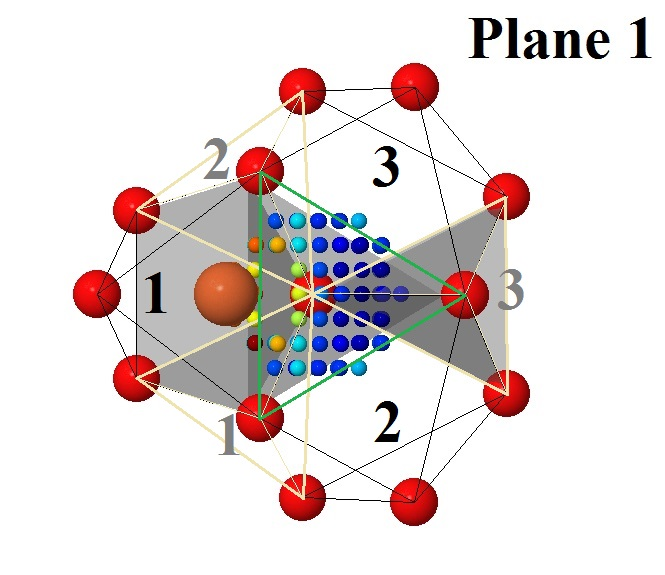
\includegraphics[width=1\linewidth]{1_color.jpg}}
\end{minipage}
\hfill
\begin{minipage}[h]{0.5\linewidth}
\center{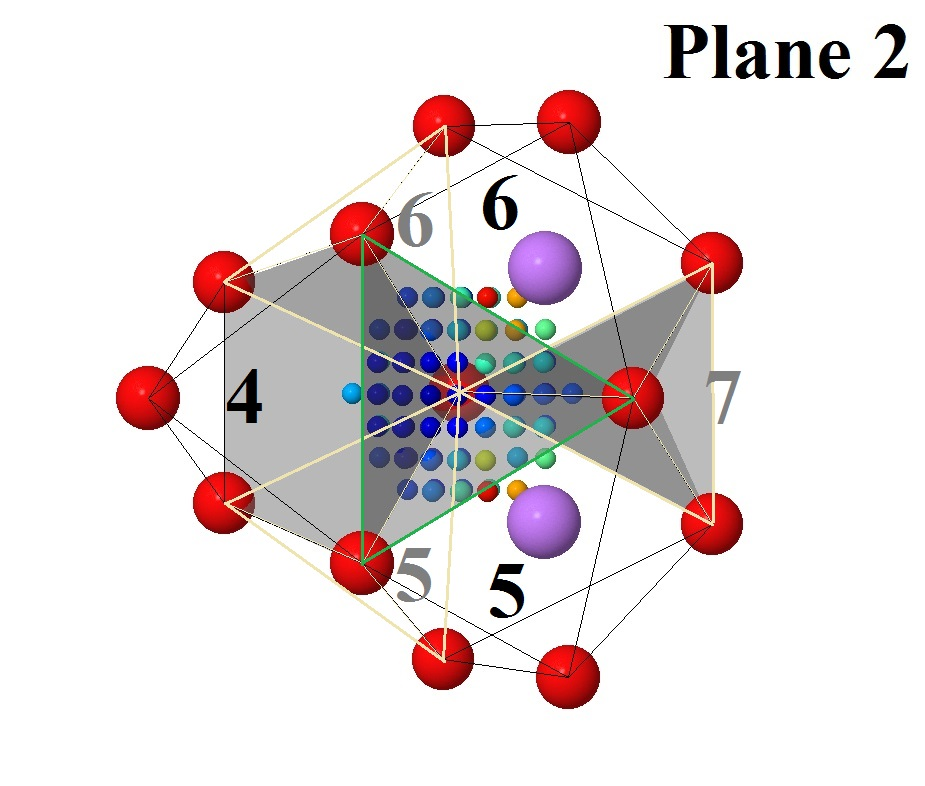
\includegraphics[width=1\linewidth]{2_color.jpg}} 
\end{minipage}
\caption{ Polyhedra around O$_1$(-0.046, 0.125, 0.147) }
\label{PH1c}
\end{figure}

 For different polyhedra the full-relaxation energy study of hydrogen atoms were performed (except num.1, 5 and 6 black near the iron and lithium atoms due to theirs hight equilibrium energy). The information about equilibrium energy of hydrogen in different positionin compared to a more stable position (num. 4 grey polyhedra) is given in the Table \ref{energy1}. There can be clear seen the advantageous position of hydrogen in defective structure: in case of tetrahedral it is fourth tetrahedral. In this situation hydrogen atom moves to the edge of tetrahedral with number three (between two atoms of oxygen - it is clear seen in fig.\ref{4to3}) and has the lower energy compared with other hydrogen positions. The similar movement but in direction to the face of tetrahedral with number 3 can be observed for hydrogen in 2 and 3 black number octahedral, 3 and 7 grey number tetrahedral. The case of movement from 7 tetrahedral to 3 tetrahedra is provided in fig.\ref{7to3}.  So, these hydrogen atoms have low energy. Hydregen atoms from octahedral with number 4 and tetrahedrals with 1, 2, 5, 6 and 8 numbers have the higer energy. In these cases atoms from 1 and 2 tetrahedral positions remove to 5 and 6 tetrahedrals, respectively. Hydrogen atoms from 5, 6 and 8 tetrahedral positions move to interfaces with 4 black number of octahedral, and, in turn, atom of hydrogen from 4 black number of octahedral removes to edge with 8 grey number of tetrahedral, Table \ref{energy1}.

\begin{figure}[H]
\begin{minipage}[h]{0.3\linewidth}
\center{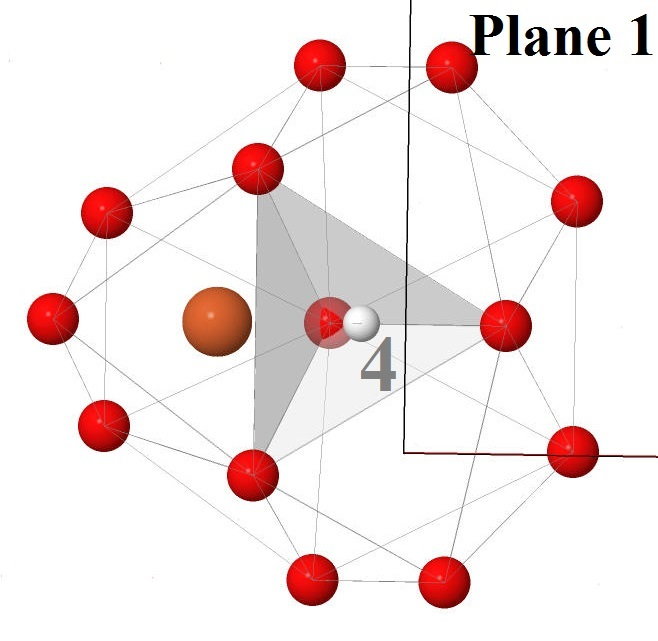
\includegraphics[width=1\linewidth]{4i1.jpg}}
\end{minipage}
\hfill
\begin{minipage}[h]{0.3\linewidth}
\center{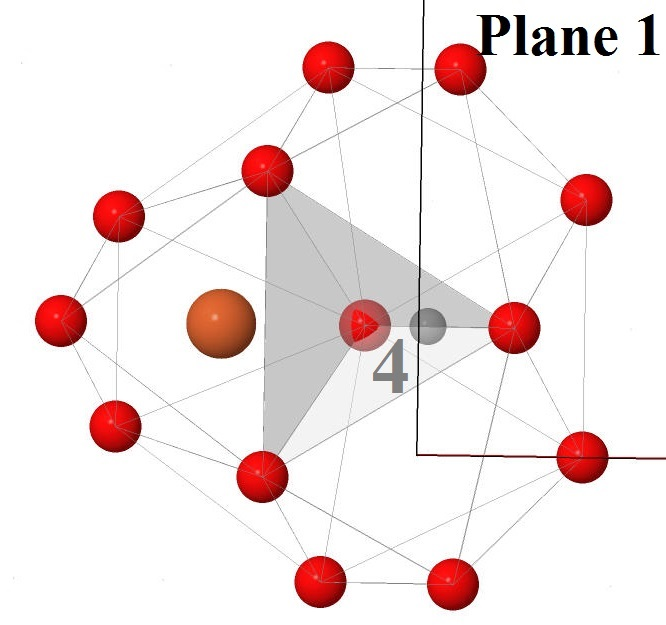
\includegraphics[width=1\linewidth]{4o1.jpg}} 
\end{minipage}
\hfill
\begin{minipage}[h]{0.3\linewidth}
\center{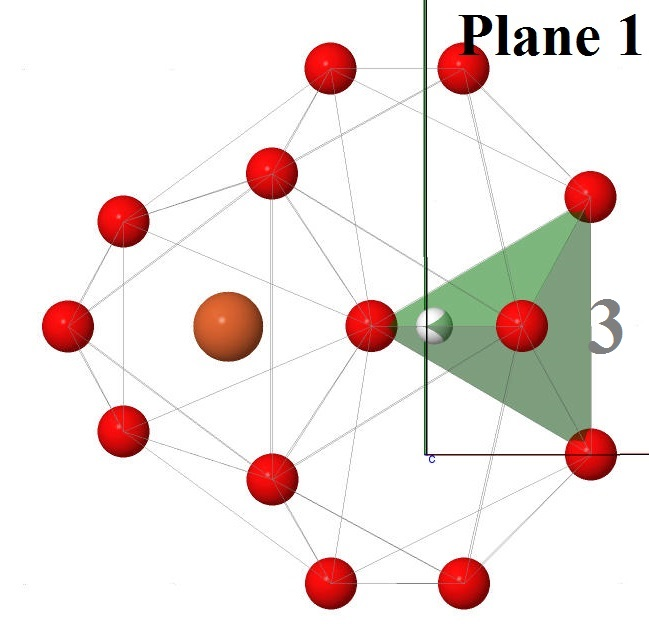
\includegraphics[width=1\linewidth]{4o2.jpg}} 
\end{minipage}
\caption{Movement of hydrogen atom from 4 grey number of tetrahedral position to 3 number tetrahedral position - more stable position: first picture - before relaxation; second and third - after relaxationin in plane 1}
\label{4to3}
\end{figure}

\begin{figure}[H]
\begin{minipage}[h]{0.5\linewidth}
\center{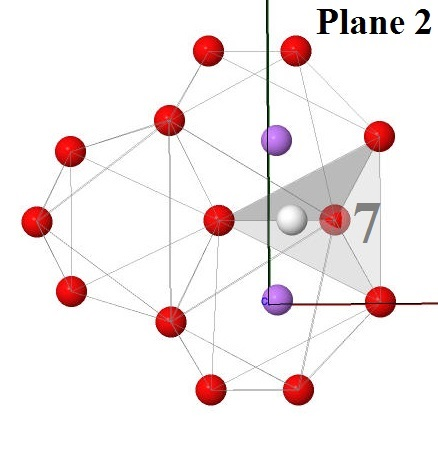
\includegraphics[width=1\linewidth]{7i1.jpg}}
\end{minipage}
\hfill
\begin{minipage}[h]{0.5\linewidth}
\center{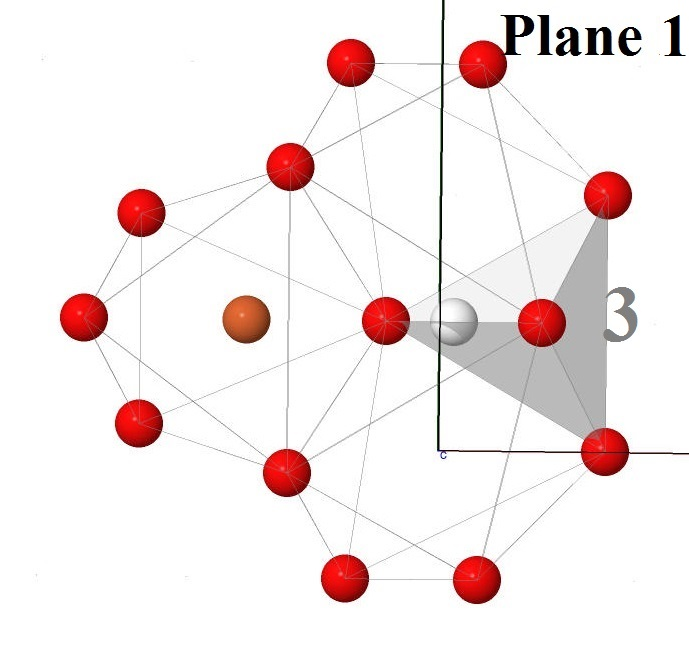
\includegraphics[width=1\linewidth]{7o1.jpg}} 
\end{minipage}
\vfill
\begin{minipage}[h]{0.5\linewidth}
\center{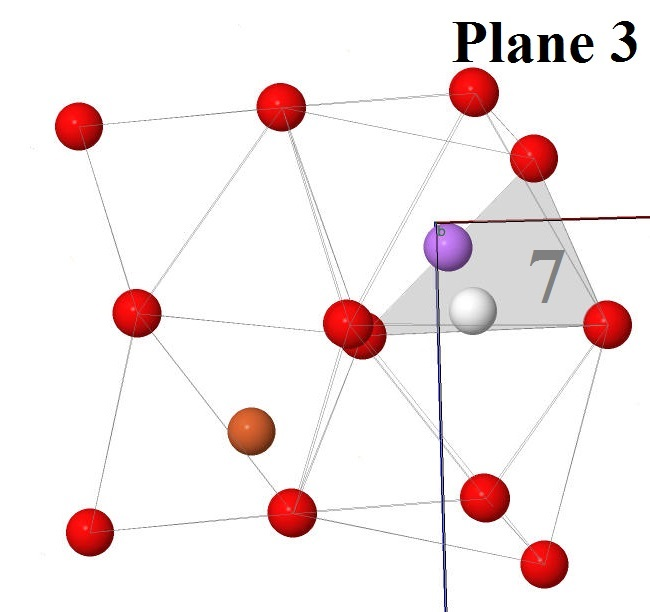
\includegraphics[width=1\linewidth]{7i2.jpg}} 
\end{minipage}
\hfill
\begin{minipage}[h]{0.5\linewidth}
\center{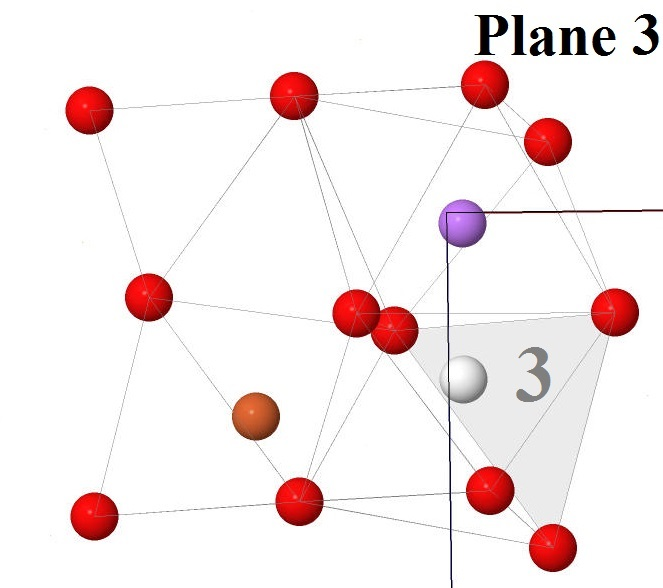
\includegraphics[width=1\linewidth]{7o2.jpg}} 
\end{minipage}
\caption{Movement of hydrogen atom from 7 grey number of tetrahedral position to 3 number tetrahedral position - one of more stable position: pictures on the left side - before relaxation; pictures in the right side - after relaxation in plane 1, 2 and 3}
\label{7to3}
\end{figure}

\begin{table}[H]
\scriptsize{
\caption{Energy of hydrogen in different polyhedra positions around first oxygen}
\label{energy1}
\begin{center}
\begin{tabular}{|c|c|c|}
\hline
& & \\
 \textbf{Polyhedra} & \textbf{Move to (direction)} & \textbf{E-E$_{3,grey}$, eV}\\ 
\hline
& & \\
 \textbf{tetrahedral}  &  & \\ 
\hline
& & \\
3 & 3 grey & 0.002 \\
\hline
& & \\
4 & 3 grey & 0.000 \\
\hline
& & \\
7 & 3 grey & 0.001 \\
\hline
& & \\
8 & 4 black & 0.419 \\
\hline
& &\\
5 & 4 black & 0.416 \\
\hline
& & \\
6 & 4 black & 0.415 \\
\hline
& &\\
1 & 4 black & 0.483 \\
\hline
& &\\
2 & 4 black & 0.432 \\
\hline
& &\\
\textbf{octahedral} & & \\
\hline
& & \\
2 & 3 grey & 0.003 \\
\hline
& &  \\
3 & 3 grey & 0.002 \\
\hline
& & \\
4 & 4 black & 0.420 \\
\hline
\end{tabular}
\end{center}
}
\end{table}

Thus, using results from Table \ref{energy1} I can provide some conclusions:

1. More stable position of hydrogen in defective LFP structure is observed in the bond between two ohygen of tetrahedral with phosphorus vacamcy.

2. The hydrogen atoms in the face of phosphorus defective tetrahedra have low formation energy.

3. Other positions, which provide low energy during first non-ralaxation steps, attempt to move to the face of 4 black number and have related high formation energy.

\section{Term Early research project}

Next stage of investigating the hydrogen defects in system of LiFePO$_4$ is the study of the hydrogen distribution around second oxygen in phosphorus-defective tetrahedral with presence of hydrogen in relevant position corresponding to second oxygen (from first step of study). In this term the energetical features of hydrogens are noted in fig.\ref{HinO1and2}. There can be clear seen that hydrogen atoms inside the tetrahedral with phosphorus defect have lower energy in comparison with other outside hydrogens (for example, near iron atom in Plane 2 picture).

\begin{figure}[H]
\begin{minipage}[h]{0.5\linewidth}
\center{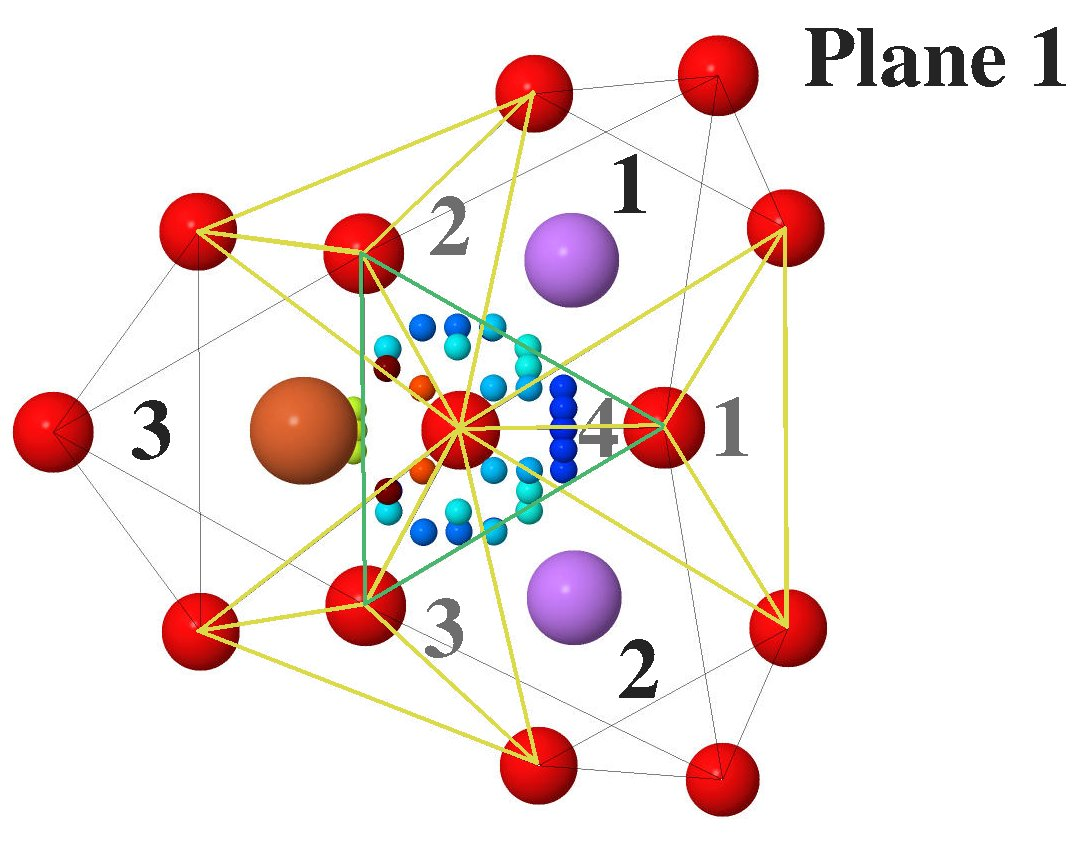
\includegraphics[width=1\linewidth]{2OPlane1CUT4.jpg}}
\end{minipage}
\hfill
\begin{minipage}[h]{0.5\linewidth}
\center{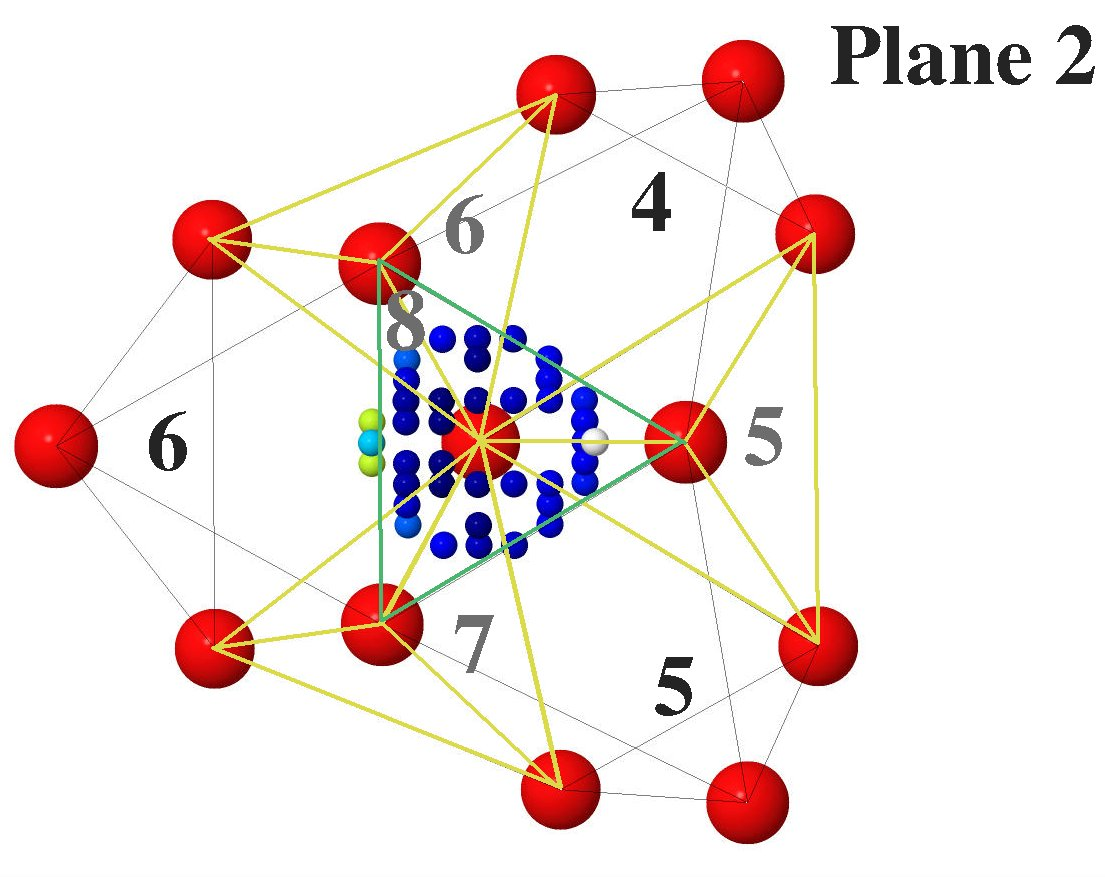
\includegraphics[width=1\linewidth]{2OPlane2CUT4.jpg}} 
\end{minipage}
\caption{Hydrogen distribution around second oxygen in phosphorus-defective tetraherdal (8 grey number)}
\label{HinO1and2}
\end{figure}

\begin{table}[H]
\scriptsize{
\caption{Energy of hydrogen in different polyhedra positions around second oxygen}
\label{energy2}
\begin{center}
\begin{tabular}{|c|c|c|}
\hline
& & \\
 \textbf{Polyhedra} & \textbf{Move to (direction)} & \textbf{E-E$_{5,black}$, eV}\\ 
\hline
& & \\
 \textbf{tetrahedral}  &  & \\ 
\hline
& & \\
8 & b/t 6\&8 grey & 0.0007 \\
\hline
& & \\
7 & 7 grey & 0.0008 \\
\hline
& & \\
6 & b/t 6\&8 grey & 0.0011 \\
\hline
& & \\
3 & 6 grey & 0.0011 \\
\hline
& &\\
2 & 7 grey & 0.0012 \\
\hline
& & \\
4 & 1 grey & 0.7166 \\
\hline
& &\\
1 & 1 grey & 0.7185 \\
\hline
& &\\
5 & 1 grey & 0.7185 \\
\hline
& &\\
\textbf{octahedral} & & \\
\hline
& & \\
\textbf{5} & \textbf{7 grey} & \textbf{0.0000} \\
\hline
& &  \\
4 & 6 grey & 0.0003 \\
\hline
& & \\
1 & 7 grey & 0.0003 \\
\hline
& & \\
2 & 6 grey & 0.0007 \\
\hline
& & \\
6 & b/t 6\&8 grey & 0.0022 \\
\hline
\end{tabular}
\end{center}
}
\end{table}

\begin{figure}[H]
\begin{minipage}[h]{0.5\linewidth}
\center{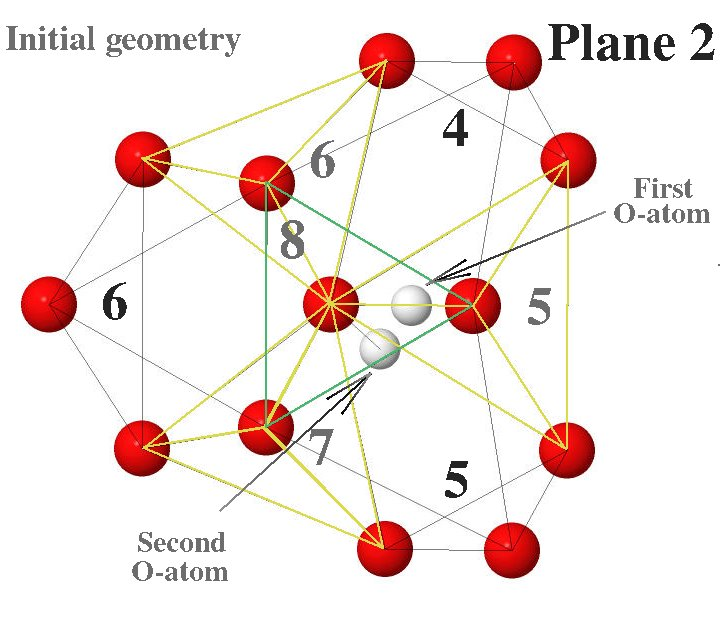
\includegraphics[width=1\linewidth]{2O5blackinitial.jpg}}
\end{minipage}
\hfill
\begin{minipage}[h]{0.5\linewidth}
\center{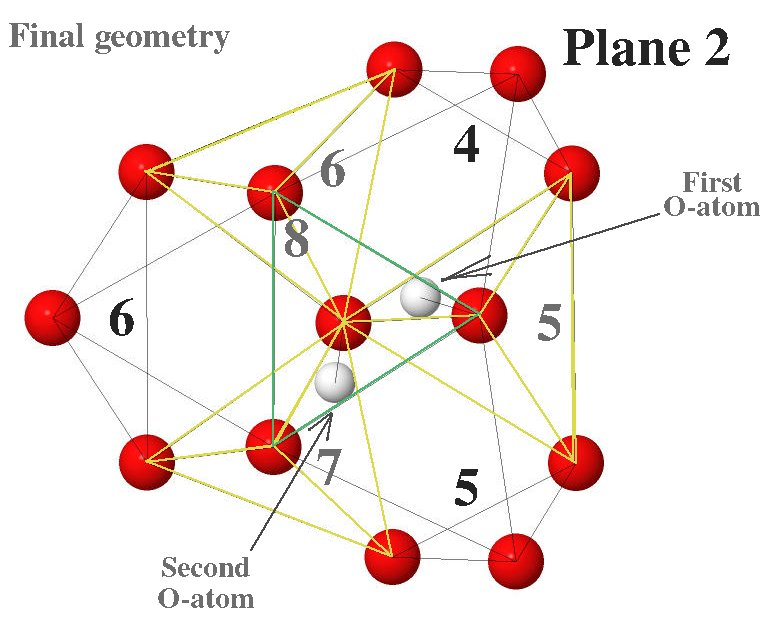
\includegraphics[width=1\linewidth]{2O5blackfinal.jpg}} 
\end{minipage}
\caption{Hydrogen distribution around second oxygen in phosphorus-defective tetraherdal }
\label{O2Finitialfinal}
\end{figure}

\section{Distribution of hydrogen around third oxygen atom}

\begin{figure}[H]
\begin{minipage}[h]{0.5\linewidth}
\center{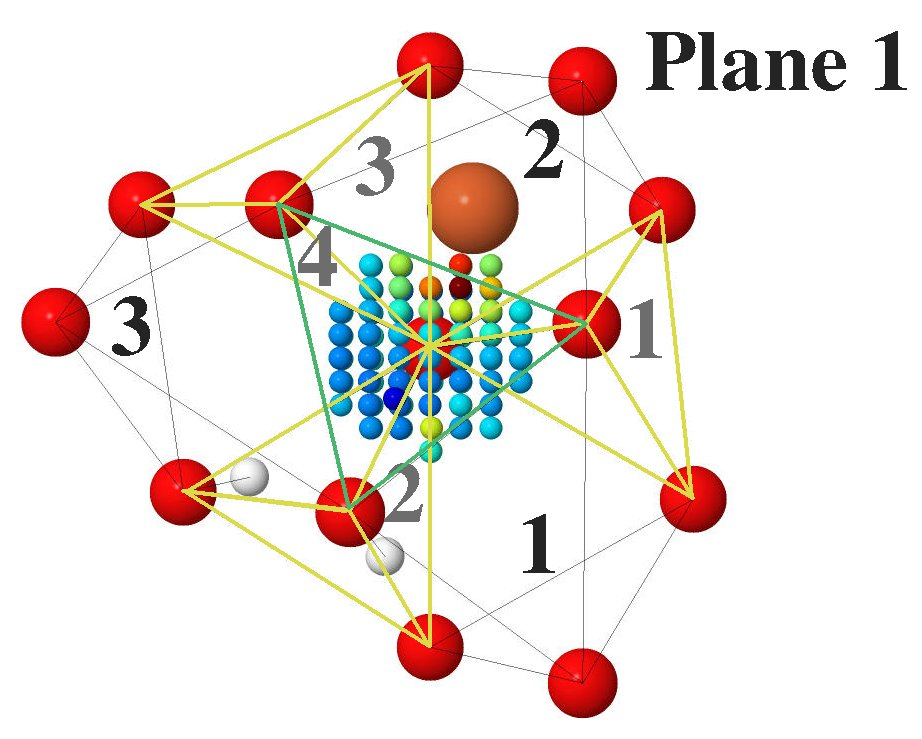
\includegraphics[width=1\linewidth]{3OPlane1.jpg}}
\end{minipage}
\hfill
\begin{minipage}[h]{0.5\linewidth}
\center{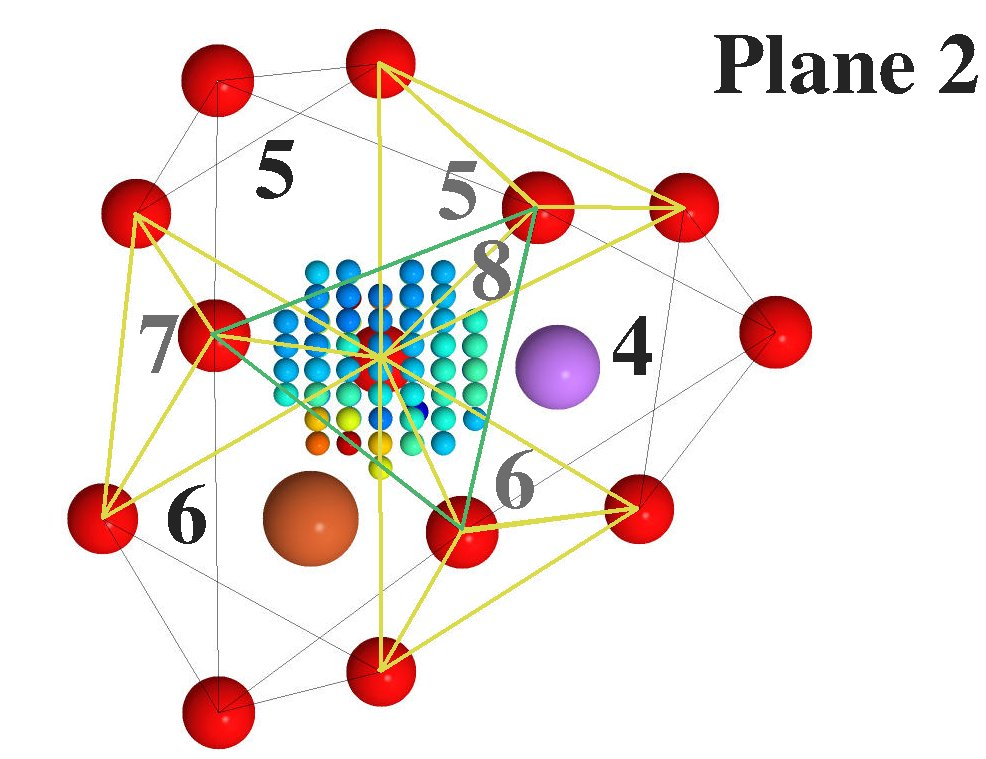
\includegraphics[width=1\linewidth]{3OPlane2.jpg}} 
\end{minipage}
\caption{Hydrogen distribution around third oxygen in phosphorus-defective tetraherdal (2 grey number)}
\label{HinO1,2and3}
\end{figure}

\begin{table}[H]
\scriptsize{
\caption{Energy of hydrogen in different polyhedra positions around second oxygen}
\label{energy3}
\begin{center}
\begin{tabular}{|c|c|c|}
\hline
& & \\
 \textbf{Polyhedra} & \textbf{Move to (direction)} & \textbf{E-E$_{2,black}$, eV}\\ 
\hline
& & \\
 \textbf{tetrahedral}  &  & \\ 
\hline
& & \\
2 & b/t 2grey\&3black & 0.512 \\
\hline
& & \\
4 & 2 grey & 0.512 \\
\hline
& & \\
1 & 1 black & 0.514 \\
\hline
& & \\
6 & b/t 2grey\&3black & 0.512 \\
\hline
& &\\
3 & 3 black & 0.514 \\
\hline
& & \\
8 & 5 black & 0.734 \\
\hline
& &\\
7 & 5 black & 0.740 \\
\hline
& &\\
5 & 5 black & 0.902 \\
\hline
& &\\
\textbf{octahedral} & & \\
\hline
& & \\
\textbf{5} & \textbf{7 grey} & \textbf{0.0000} \\
\hline
& &  \\
2 & b/t 2grey\&3black & 0.000 \\
\hline
& & \\
6 & 5 black & 0.190 \\
\hline
& & \\
1 & b/t 2grey\&4grey & 0.511 \\
\hline
& & \\
3 & b/t 2grey\&3black & 0.514 \\
\hline
& & \\
4 & b/t 2grey\&3black & 0.515 \\
\hline
& & \\
5 & 5 black & 0.738 \\
\hline
\end{tabular}
\end{center}
}
\end{table}

\begin{figure}[H]
\begin{minipage}[h]{0.5\linewidth}
\center{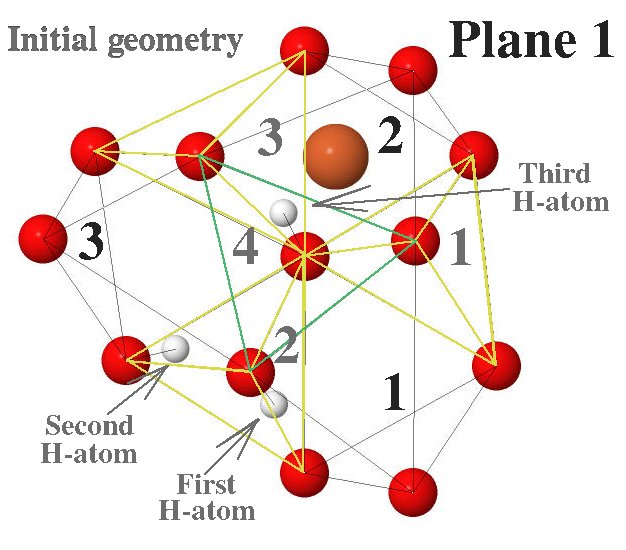
\includegraphics[width=1\linewidth]{3Obefore2black.jpg}}
\end{minipage}
\hfill
\begin{minipage}[h]{0.5\linewidth}
\center{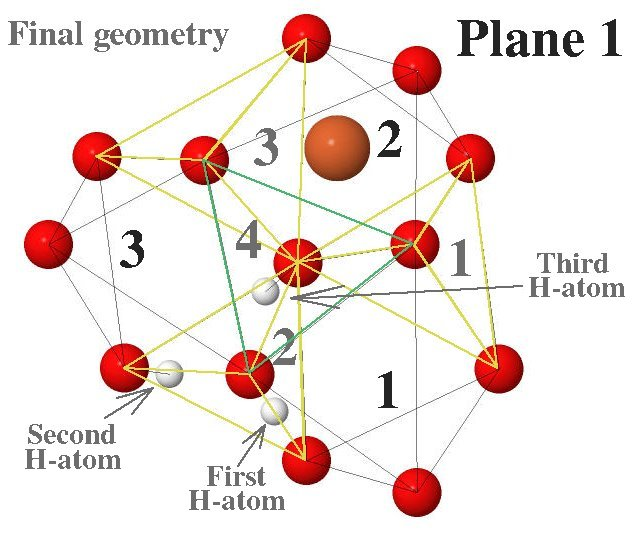
\includegraphics[width=1\linewidth]{3Oafter2black.jpg}} 
\end{minipage}
\caption{Hydrogen movement to stable position around third oxygen in phosphorus-defective LFP}
\label{O3Finitialfinal}
\end{figure}


\begin{thebibliography}{9}
\bibitem{LFP} Whittingham, M. Stanley. "Lithium batteries and cathode materials." Chemical reviews 104.10 (2004): 4271-4302.

\bibitem{LiFe} Hu, Boyang, and Guohua Tao. "Molecular dynamics simulations on lithium diffusion in LiFePO$_4$: the effect of anti-site defects." Journal of Materials Chemistry A 3.40 (2015): 20399-20407.

\bibitem{Livac} Tealdi, Cristina, Clelia Spreafico, and Piercarlo Mustarelli. "Lithium diffusion in Li$_{1-x}$FePO$_4$: the effect of cationic disorder." Journal of Materials Chemistry 22.47 (2012): 24870-24876.

\bibitem{def} Bai, Quan, and D. L. Kohlstedt. "Substantial hydrogen solubility in olivine and implications for water storage in the mantle." Nature 357.6380 (1992): 672.

\bibitem{def1} Amisse, Robin, et al. "Singular structural and electrochemical properties in highly defective LiFePO$_4$ powders." Chemistry of materials 27.12 (2015): 4261-4273.

\bibitem{oh} Wright, Kate, and C. R. A. Catlow. "A computer simulation study of (OH) defects in olivine." Physics and Chemistry of Minerals 20.7 (1994): 515-518.

\bibitem{morgan} Morgan, D., and A. Van der Ven. "D. Morgan, A. Van der Ven, and G. Ceder, Electrochem. Solid-State Lett. 7, A30 (2004)." Electrochem. Solid-State Lett. 7 (2004): A30.

\bibitem{bgap}  Zhou, Fei, et al. "The electronic structure and band gap of LiFePO$_4$ and LiMnPO$_4$." Solid State Communications 132.3-4 (2004): 181-186.

\bibitem{mineral} Qin, Tian, et al. "Ab initio study of water speciation in forsterite." APS Meeting Abstracts. 2018.
\end{thebibliography}
\end{document}
